\section*{Appendices}
\begin{appendices}
	
% ===================================================================================================
%                                                 |                                                 |
%                                                 |                                                 |
% -------------------------------------------- SECTION ---------------------------------------------|
%                                                 |                                                 |
%                                                 |                                                 |
% ===================================================================================================
\section{Industrial robot energy consumption support data}\label{sec:app_robot_ener_consumption}
According to \cite{montaqim2015} and available press releases of different robotic companies \cite{fanuc2015, yaskawa2014, ABB2015}, the approximate distribution of the industrial robot install base per manufacturer is shown in Fig.~\ref{fig:manufacturers_pie}.
% ---
\begin{figure}[!ht]
	\centering
	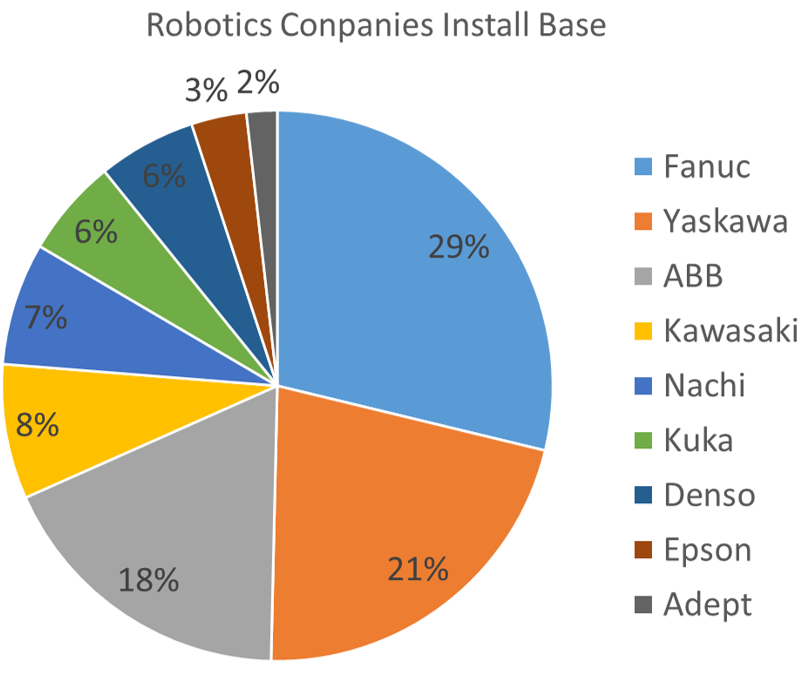
\includegraphics[width=0.95\columnwidth]{fig/manufacturers}
	\caption{Percentage of installed industrial robots per manufacturer}
	\label{fig:manufacturers_pie}
\end{figure}
% ---
Since Fanuc, Yaskawa, and ABB make for two-thirds of the total install base of industrial robots, we took the power consumption of the robots from those manufacturers to estimate the total power consumption. 
After surveying the datasheets for their robot portfolio, the average power consumption for each model was estimated. Additionally, every manufacturer classifies their robots according to one or more possible applications, which can be grouped into the application categories defined by the IFR. The average power consumption was calculated for every application using the values reported in the robot datasheets. Finally, the power consumption for each category was computed as a weighted average based on the companies' market share percentage (assuming that 68 \% is the total number of robots)\footnote[1]{These numbers should be used with discretion since there is no available information on which are the most common installed robot models. This information may change the estimation.}. The estimated power consumption per robot application is shown in Fig.~\ref{fig:ir_average_power}.
%---
\begin{figure}[h]
	\centering
	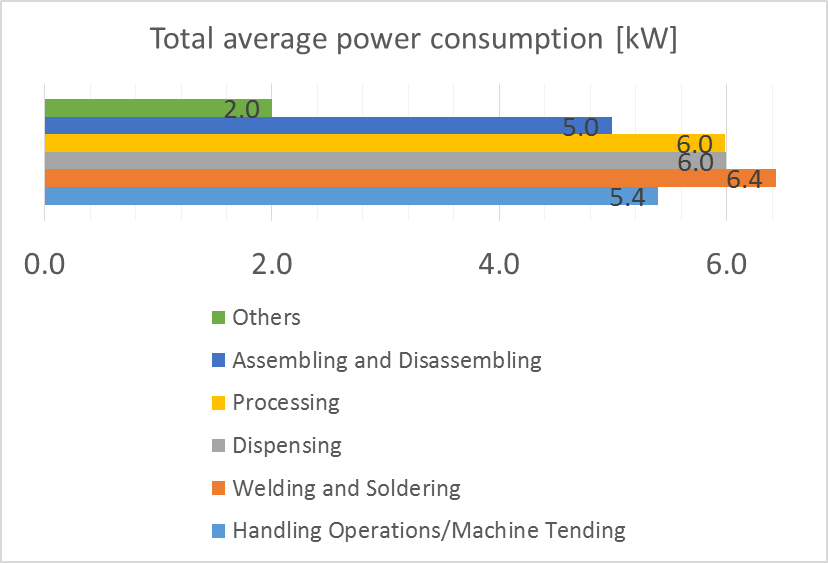
\includegraphics[width=0.95\columnwidth]{fig/industrial_robots_average_power_per_category}
	\caption{Average power consumption of industrial robots per category.}
	\label{fig:ir_average_power}
\end{figure}
%---
Using these numbers and the estimated operational stock of industrial robots reported in \cite{statista_ir_operational_stock} and by the International Federation of Robotics (see Fig.~\ref{fig:ir_stock}), the estimated worldwide industrial robot energy consumption was computed and shown in Fig.~\ref{fig:ir_energy}.
% ===================================================================================================
%                                                 |                                                 |
%                                                 |                                                 |
% -------------------------------------------- SECTION ---------------------------------------------|
%                                                 |                                                 |
%                                                 |                                                 |
% ===================================================================================================
\section{Collaborative robots}\label{sec:app_cobot_ener_consumption}
To approximate the energy consumption of cobots we looked at the power consumption per payload of various manufacturers, see Fig.~\ref{fig:cobot_watt_per_kg} resulting in an average power consumption of approximately 40 W. Together with a typical power consumption of the robot controller of 60 W \cite{Heredia2023BreakingEnergyConsumption}, we consider a total of 100 W power demand. Similar to the industrial robots, the worldwide energy consumption was calculated assuming a 24/7 operation.
%---
\begin{figure}[h]
	\centering
	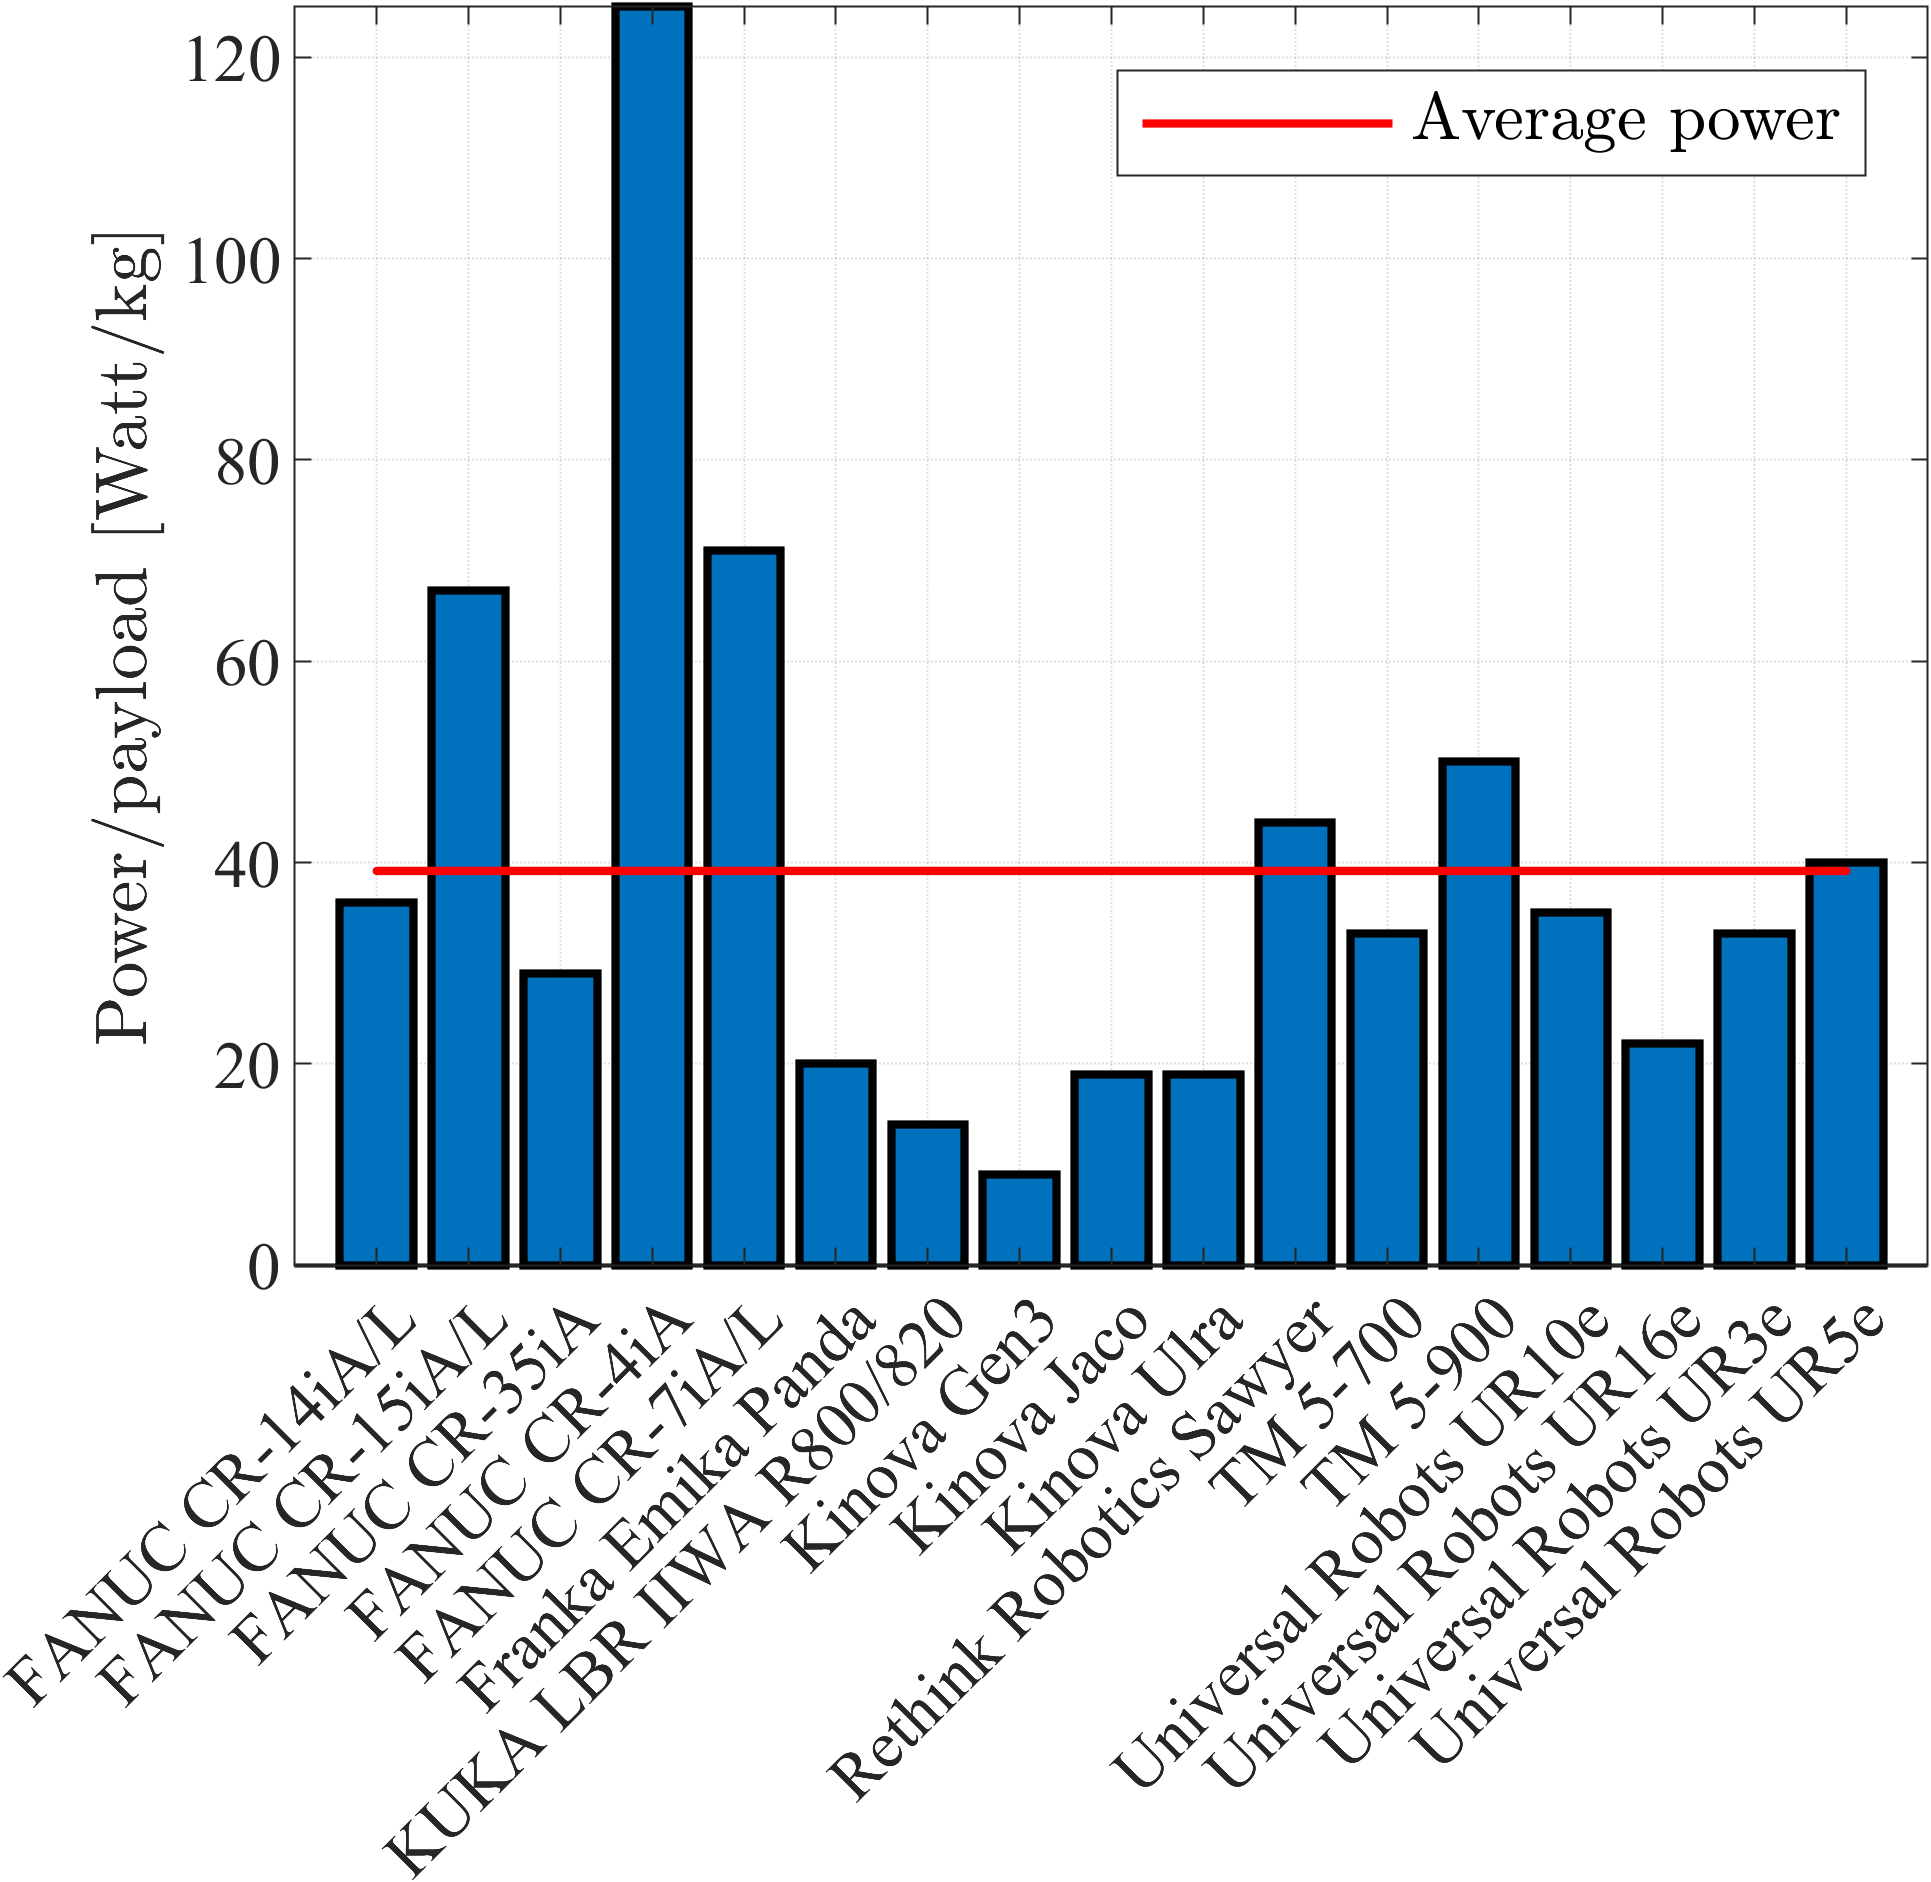
\includegraphics[width=0.95\columnwidth]{cobot_watt_per_kg.png}
	\caption{Power consumption per payload for different cobots.}
	\label{fig:cobot_watt_per_kg}
\end{figure}
%---

\end{appendices}


